\scanpage{173}
\mspage{31}

faisceau abélien \inserted{constant} $F$ sur $\unsure{\mathscr X|\mathcal X}$, on a $H^i(\mathscr X,F)=0$ pour $i>0$. On procède par récurrence sur $i$, c'est déjà fait pour $i=1$. \deleted{On} Supposons que ce soit prouvé pour les $j<i$ \inserted{\unsure{$i$ fixé}} \deleted{\unsure{et pour}} pour \unsure{tt} topos \deleted{\unsure{local}} \uline{tot $0$-connexe}. Soit $\xi\in H^i(\mathscr X,F)$, soit $U\to e$ épi tel que $\xi\mid U=0$, \deleted{\unsure{et}} considérons la suite spectrale

\[
\deleted{\unsure{E_1}}E_{\unsure{2|1}}^{pq}=H^{\deleted{\unsure{q}}\unsure{p}}\bigl(\unsure{C|\check C}(U^{\unsure{*|p}},\unsure{\mathcal H|\mathscr H}^{\deleted{\unsure{p}}q}F)\bigr)\Longrightarrow H^*(\mathscr X,F)
\]

\deleted{On a par hyp. de récurrence, les composantes} On a par hypothèse tot. $0$-connexe

\[
\pi_0(U^{\unsure{q|p}})\simeq\pi_0(U)^q,\tag*{$(\alpha)$}
\]

et les composantes connexes de $U^q$ sont \deleted{$0$-connexes, ce \unsure{qu'}} tot $0$-\unsure{asph.}, donc par hypothèse de récurrence

\[
E_1^{pq}=0\quad\text{si }0<q<i,
\]

donc on trouve une suite exacte

\figure{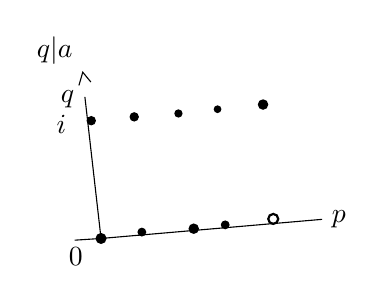
\begin{tikzpicture}[x=.54cm,y=.54cm]
\draw (0,0)--(-.38,3.33);
\draw (-.52,3.60)--(-.43,3.91)--(-.24,3.68);
\node[above left] at (-.44,3.86) {$\unsure{q|a}$};
\draw (-.62,-.04)--(0,0)--(5.2,.45) node[right] {$p$};
\node[below left] at (-.20,.02) {$0$};
\node[left] at (-.59,2.69) {$i$};
\node[left] at (-.40,3.27) {$\deleted{\unsure{q}}$};
\fill (0,0) circle (2pt) (.96,.15) circle (1.6pt) (2.18,.23) circle (1.9pt) (2.92,.32) circle (1.6pt);
\draw[thick] (4.05,.46) circle (1.8pt);
\fill (-.23,2.77) circle (1.7pt) (.78,2.86) circle (1.7pt) (1.82,2.94) circle (1.5pt) (2.74,3.04) circle (1.4pt) (3.81,3.15) circle (1.9pt);
\end{tikzpicture}}

\diagram{\begin{tikzcd}[ampersand replacement=\&]
0\arrow[r] \& H^{\deleted{\unsure{p}}i}(C(U^{*},F))\arrow[r] \& H^{\deleted{\unsure{p}}i}(\mathscr X,F)\arrow[r] \& H^0\bigl[\underbrace{H^{\deleted{\unsure{p}}i}(U^{*},F)}_{\substack{\text{complexe}\\\text{cosimplicial}\\\text{pour }p}}\bigr)\\
\&\&\rotatebox{90}{$\in$}\&\Vert\\
\&\&\xi\&\operatorname{Ker}\bigl(H^i(U,F)\rightrightarrows H^i(U^2,F)\bigr)
\end{tikzcd}}

\unsure{$1$} \unsure{de sorte} Par hypothèse sur $U$, l'image de $\xi$ dans le troisième terme est nulle, donc $\xi$ appartient au premier terme. Mais \inserted{par $(\alpha)$,} le complexe $C(U^\bullet,F)$ est \deleted{\unsure{celui de}} le complexe \uline{trivial} des puissances de $I=\pi_0(U)$, à coeff. \inserted{dans $M$} (car $F=M_{\mathscr X}$). Sa cohomologie

% archive sheet number: 173
